\section{Data Understanding}
\label{sec:data-understanding}

\subsection{Dataset Overview}

The dataset used in this project is the \textbf{Crimes 2001--Present} dataset published by the Chicago Police Department via the Socrata Open Data Portal\footnote{\url{https://data.cityofchicago.org/Public-Safety/Crimes-2001-to-Present/ijzp-q8t2}}. It contains all reported crime incidents in Chicago from 2001 to early 2026.

\begin{table}[H]
\centering
\caption{Dataset Overview}
\label{tab:dataset-overview}
\begin{tabular}{ll}
\toprule
\textbf{Attribute} & \textbf{Value} \\
\midrule
Source & Chicago Data Portal (Socrata SODA API) \\
Records & 8,549,662 \\
Columns & 22 \\
Uncompressed Size & $\sim$1.9 GB (CSV) \\
HDFS Size (Parquet+Snappy) & 509 MB \\
Primary Key & \texttt{id} \\
Target Variable & \texttt{arrest} (Boolean) \\
Geospatial Fields & \texttt{latitude}, \texttt{longitude} \\
Temporal Fields & \texttt{date}, \texttt{updated\_on}, \texttt{year} \\
Time Span & 2001 -- 2026 \\
Police Districts & 24 \\
Community Areas & 77 \\
Crime Types & 34 primary categories \\
\bottomrule
\end{tabular}
\end{table}

\subsection{Schema Description}

The dataset contains 22 columns covering crime identification, categorisation, temporal, geospatial, and administrative attributes. The detailed schema is presented in Table~\ref{tab:schema}.

\begin{table}[H]
\centering
\caption{Crimes Dataset Column Schema}
\label{tab:schema}
\begin{tabularx}{\textwidth}{llX}
\toprule
\textbf{Column} & \textbf{Type} & \textbf{Description} \\
\midrule
\texttt{id} & BIGINT & Unique record identifier \\
\texttt{case\_number} & VARCHAR(20) & Case reference number \\
\texttt{date} & TIMESTAMP & Incident timestamp \\
\texttt{block} & VARCHAR(200) & Address block \\
\texttt{iucr} & VARCHAR(10) & Illinois Uniform Crime Reporting code \\
\texttt{primary\_type} & VARCHAR(50) & Crime category \\
\texttt{description} & VARCHAR(300) & Detailed crime description \\
\texttt{location\_description} & VARCHAR(100) & Location context \\
\texttt{arrest} & BOOLEAN & \textbf{Target variable} \\
\texttt{domestic} & BOOLEAN & Domestic incident flag \\
\texttt{beat} & VARCHAR(10) & Police beat area \\
\texttt{district} & SMALLINT & Police district (1--25) \\
\texttt{ward} & SMALLINT & City ward \\
\texttt{community\_area} & SMALLINT & Community area (1--77) \\
\texttt{fbi\_code} & VARCHAR(10) & FBI UCR code \\
\texttt{x\_coordinate} & INTEGER & X projection coordinate \\
\texttt{y\_coordinate} & INTEGER & Y projection coordinate \\
\texttt{year} & SMALLINT & Incident year \\
\texttt{updated\_on} & TIMESTAMP & Last update timestamp \\
\texttt{latitude} & DOUBLE & GPS latitude \\
\texttt{longitude} & DOUBLE & GPS longitude \\
\texttt{location} & VARCHAR(300) & Raw location string \\
\bottomrule
\end{tabularx}
\end{table}

\subsection{Data Quality Assessment}

\subsubsection{Class Balance}

The target variable \texttt{arrest} exhibits significant class imbalance:

\begin{itemize}
    \item \textbf{TRUE (arrest made)}: 2,145,230 records (25.09\%)
    \item \textbf{FALSE (no arrest)}: 6,404,432 records (74.91\%)
\end{itemize}

This $\sim$1:3 ratio means that standard accuracy-based metrics can be misleading. We prioritise AUC-PR (precision-recall) over AUC-ROC for model evaluation.

\subsubsection{Missing Values}

Several columns contain missing values that require handling:

\begin{itemize}
    \item \textbf{Coordinates} (\texttt{latitude}, \texttt{longitude}): 96,553 nulls ($\sim$1.1\%) — records excluded from ML training.
    \item \texttt{community\_area}: 613,725 nulls ($\sim$7.2\%) — imputed with -1.
    \item \texttt{district}: 47 nulls — imputed with -1.
    \item Categorical columns (\texttt{primary\_type}, \texttt{iucr}, \texttt{location\_description}, \texttt{beat}): filled with \texttt{"Unknown"}.
\end{itemize}

\subsubsection{Geospatial Validation}

All recorded coordinates fall within the valid Chicago bounding box: latitude $[41.6, 42.1]$, longitude $[-87.9, -87.5]$. No out-of-bounds records were detected.

\subsection{Exploratory Data Analysis}

Seven exploratory queries were executed via PySpark to uncover crime patterns. Results are summarised in Table~\ref{tab:eda-insights}.

\begin{table}[H]
\centering
\caption{EDA Insights Summary}
\label{tab:eda-insights}
\begin{tabularx}{\textwidth}{cX}
\toprule
\textbf{Q\#} & \textbf{Key Finding} \\
\midrule
Q1 & Arrest rate varies 2.25$\times$ across districts: District 11 highest (40.89\%), District 16 lowest (18.19\%). \\
Q2 & THEFT (1.82M) and BATTERY (1.56M) dominate — top 5 types represent $>$65\% of all incidents. \\
Q3 & Crime volume follows a diurnal pattern: peaks at 12:00 (490K) and 18:00; lowest at 5 AM (120K). \\
Q4 & Arrest rates declined from 29.21\% (2001) to $\sim$12--16\% (2020s), with a sharp drop between 2015--2016. \\
Q5 & Monthly crime volume is relatively stable ($\sim$10\% variation); February lowest, May/December highest. \\
Q6 & Wide variation across 77 community areas: from $\sim$10\% to 36.68\% (Area 23). \\
Q7 & Non-domestic incidents (26.32\%) have higher arrest rates than domestic (19.22\%). \\
\bottomrule
\end{tabularx}
\end{table}

\subsubsection{Key EDA Visualisations}

Figure~\ref{fig:eda-q1} through Figure~\ref{fig:eda-q7} present the Superset chart exports for each EDA query.

\begin{figure}[H]
    \centering
    \begin{subfigure}{0.48\textwidth}
        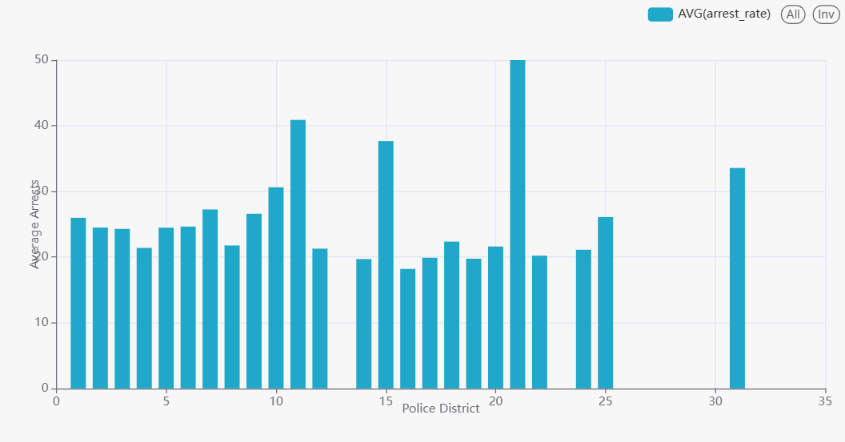
\includegraphics[width=\textwidth]{output/q1.jpg}
        \caption{Arrest Rate by District (Q1)}
        \label{fig:eda-q1}
    \end{subfigure}
    \hfill
    \begin{subfigure}{0.48\textwidth}
        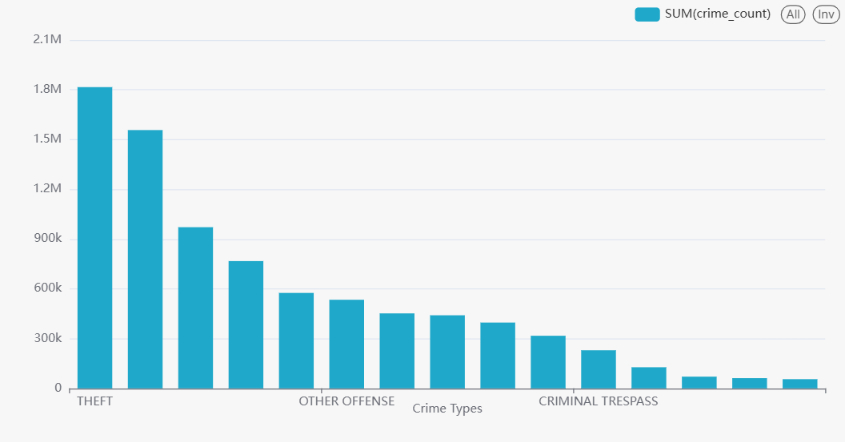
\includegraphics[width=\textwidth]{output/q2.jpg}
        \caption{Top 15 Crime Types (Q2)}
        \label{fig:eda-q2}
    \end{subfigure}
    \vspace{0.3cm}
    \begin{subfigure}{0.48\textwidth}
        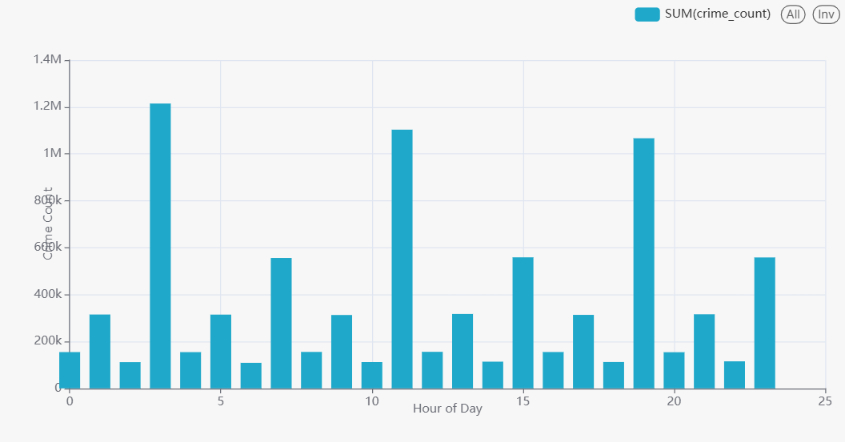
\includegraphics[width=\textwidth]{output/q3.jpg}
        \caption{Crimes by Hour (Q3)}
        \label{fig:eda-q3}
    \end{subfigure}
    \hfill
    \begin{subfigure}{0.48\textwidth}
        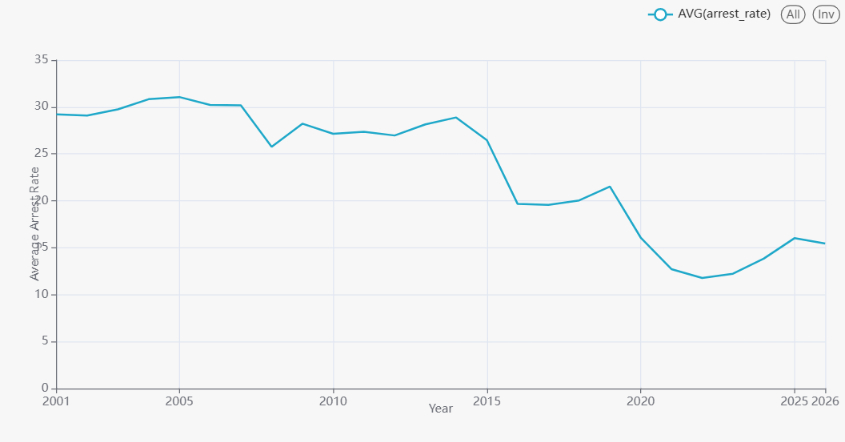
\includegraphics[width=\textwidth]{output/q4.jpg}
        \caption{Arrest Rate Trend (Q4)}
        \label{fig:eda-q4}
    \end{subfigure}
    \caption{EDA Charts 1--4}
\end{figure}

\begin{figure}[H]
    \centering
    \begin{subfigure}{0.48\textwidth}
        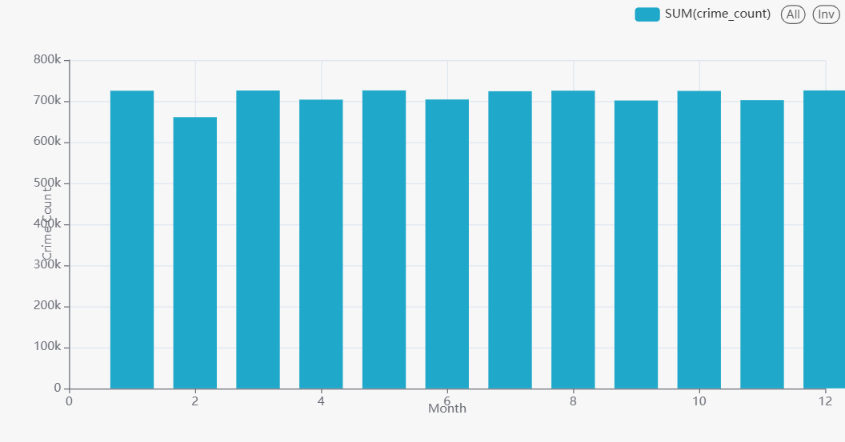
\includegraphics[width=\textwidth]{output/q5.jpg}
        \caption{Crimes by Month (Q5)}
        \label{fig:eda-q5}
    \end{subfigure}
    \hfill
    \begin{subfigure}{0.48\textwidth}
        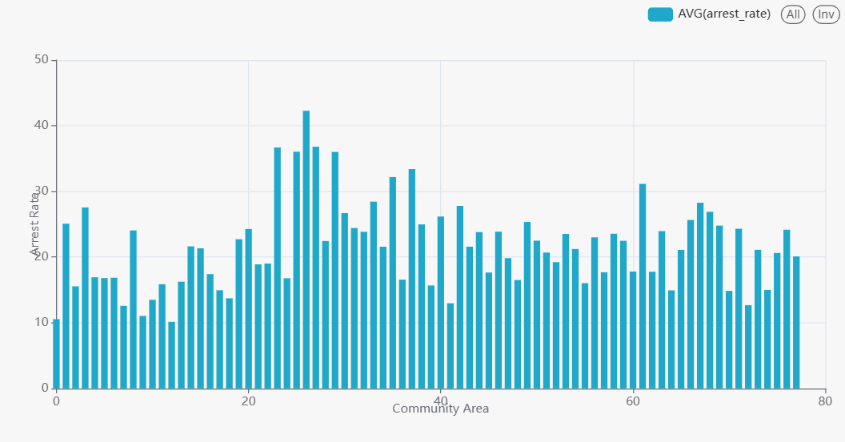
\includegraphics[width=\textwidth]{output/q6.jpg}
        \caption{Arrest Rate by Community Area (Q6)}
        \label{fig:eda-q6}
    \end{subfigure}
    \vspace{0.3cm}
    \begin{subfigure}{0.48\textwidth}
        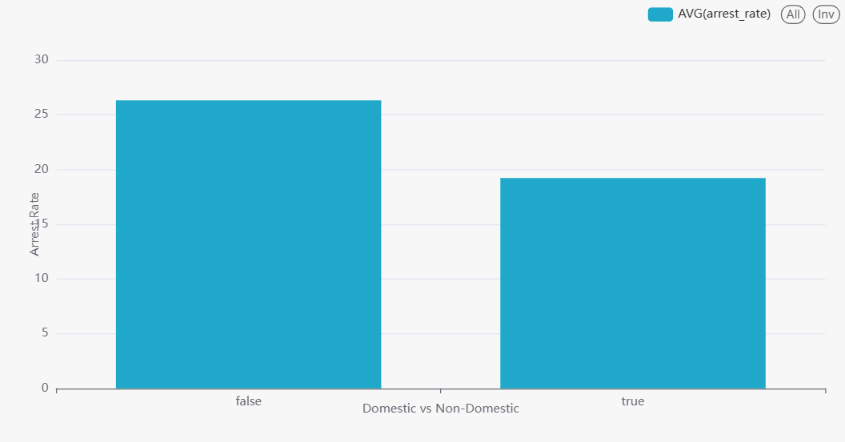
\includegraphics[width=\textwidth]{output/q7.jpg}
        \caption{Domestic vs Non-Domestic (Q7)}
        \label{fig:eda-q7}
    \end{subfigure}
    \caption{EDA Charts 5--7}
\end{figure}
